\section{引言}
\label{sec:intro}
大语言模型（LLM）在长上下文序列处理上已展现出显著能力~\citep{liu2025comprehensive,liu2025thus,mei2025survey}。
然而，标准全注意力（\textbf{FA}）机制~\citep{vaswani2017attention}的二次计算与内存复杂度，会随着上下文窗口扩大而迅速成为可扩展性的核心瓶颈。
稀疏注意力（\textbf{SA}）机制~\citep{child2019generating,zaheer2020big}通过仅关注关键 token 子集来有效缓解这一问题，从而显著降低计算开销并提升推理吞吐。

\begin{figure}[t]
  \centering
    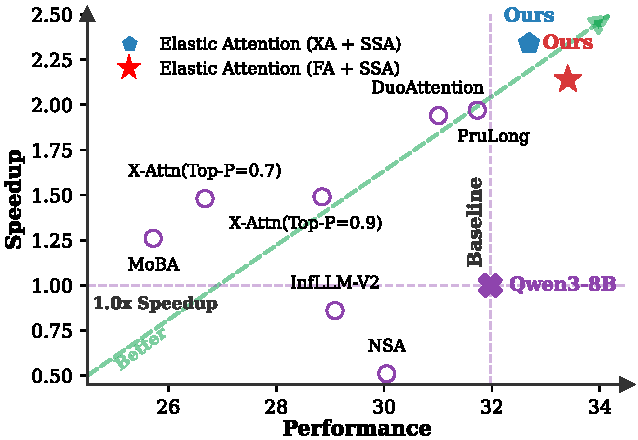
\includegraphics[width=\linewidth]{figures/speedup_vs_performance_comparison.pdf}
    \caption{Elastic Attention（我们的方法）与现有方法在 LongBench-V2~\citep{bai2024longbench2} 上的对比。“(XA+SSA)”与“(FA+SSA)”表示我们的不同配置。}
    \label{fig:intro_speedup_vs_performance}
\end{figure}

为平衡计算成本与模型质量（即接近 FA 的性能），现有方法通常采用混合建模策略，在单个模型中同时集成 SA 与 FA~\citep{zhang2025efficient,xiaoduoattention2025}。
但下游任务性能对两种注意力计算模式的占比非常敏感（见 \Cref{subsec:deployment_sparisity} 的预分析），而寻找合适占比通常需要大量任务特定验证或调参，这严重限制了方法的鲁棒性与通用性~\citep{peng2025accelerating}。

本文首先发现，下游任务可自然归纳为两类：（1）\emph{稀疏鲁棒型任务}（如摘要），在较宽稀疏范围内性能基本稳定；（2）\emph{稀疏敏感型任务}（如问答），当稀疏度超过阈值后性能显著下降。
这一观察意味着，模型无需为每个任务分别学习精细稀疏配置，而只需区分这两类任务并分配相应稀疏度。
基于此，我们提出 \emph{\textbf{Elastic Attention}}，使模型在 prefill 阶段能够自动调整整体稀疏度，以适配上述两类任务。
我们方法的核心是集成到现有 Transformer 架构中的轻量 \emph{\textbf{Attention Router}} 模块。

具体而言，Attention Router 的工作方式类似 Mixture-of-Experts~\citep{shazeer2017outrageously}：它基于输入隐状态执行按头路由，动态将每个注意力头分配到 FA 或 SA 计算模式，从而动态调整模型整体稀疏度。
Attention Router 的额外开销很小，在头维度为 128 时每层仅增加 0.27M 参数，兼顾了推理效率与计算成本。
为优化该模块，我们采用基于 Gumbel-Softmax~\citep {jang2016categorical} 的连续松弛方案，以缓解离散路由带来的训练-推理不一致问题。
同时，为稳定优化过程，我们结合 straight-through estimator（STE）~\citep{bengio2013estimating} 进行梯度传播。
推理时，同一层内不同头可以被路由到不同计算模式。
我们进一步设计了融合 kernel，使所有被路由的头能够在一次前向中并行处理。

我们在 3 个广泛使用且具有代表性的 LLM 上验证方法（Qwen3 系列~\citep{yang2025qwen3technicalreport} 与 Llama-3.1-8B-Instruct~\citep{grattafiori2024llama}），并同时考虑 Streaming~\citep{streamingllm} 与 block-sparse~\citep{guo2024blocksparse} 两种 SA 模式。
在覆盖真实任务、合成检索任务与长程推理任务的多类长上下文基准上，我们的方法不仅能学习到任务相关的稀疏分配，还在性能上稳定优于基线。
值得注意的是，这一提升在有限训练预算下即可实现：无需修改骨干模型参数，仅用 8$\times$A800 GPU 训练 12 小时。
此外，我们还对 Attention Router 进行了深入分析，包括架构设计、参数容量影响，以及详细的训练监控指标。
